\section{树构造:从 PRG 到 PRF}\label{sec:4-6}

事实证明,给定一个合适的、安全的 PRG,我们可以用一种叫做\textbf{树构造 (tree construction)}的技术来构建一个安全的 PRF。将这一结果与 \ref{sec:4-5} 节中的卢比-拉克福构造相结合,我们可以看到,我们可以基于任何一个安全 PRG 构造出一个安全的分组密码。虽然这一结果具有一定的理论意义,但这种构造并不十分高效,而且在实践中也没有被真正使用。然而,我们注意到,这种构造的一种简单推广在实际的消息认证方案中发挥着重要的作用,我们将在 \ref{subsec:6-4-2} 小节中讨论这个问题。

我们从一个定义在 $(\mathcal{S},\mathcal{S}^2)$ 上的伪随机数生成器 $G$ 开始。也就是说,$G$ 的种子空间是一个集合 $\mathcal{S}$,而输出空间是所有种子对的集合 $\mathcal{S}^2$。比如,$G$ 可以将 $n$ 比特序列拉伸为 $2n$ 比特的序列\footnote[2]{事实上,我们甚至可以从一个 PRG 开始,将 $n$ 比特的序列拉伸为 $(n+1)$ 比特,然后应用定理 \ref{theo:3-3} 中分析的$n$次串行组合构造来获得一个合适的 $G$。}。方便的做法是将其表示成$G(s) = (G_0(s),G_1(s))$;也就是说,$G_0(s)\in\mathcal{S}$ 表示 $G(s)$ 的第一个组成部分,$G_1(s)$ 表示 $G(s)$ 的第二个组成部分。我们将基于 $G$ 构造一个伪随机函数 $F$,其密钥空间为 $\mathcal{S}$,输入空间为 $\{0,1\}^\ell$(其中 $\ell$ 是一个任意的、多项式边界的值),输出空间为 $\mathcal{S}$。

我们首先定义一个算法 $G^*$,它接受 $s\in\mathcal{S}$ 和 $x=(a_1,\dots,a_n)\in\{0,1\}^n$ 作为输入,其中对于 $i=1,\dots,n$ 有 $a_i\in\{0,1\}$,输出一个元素 $t\in\mathcal{S}$,其工作原理如下:

\vspace{5pt}

\hspace*{5pt} 令 $t\leftarrow s$\\
\hspace*{26pt} 对于 $i=1,\dots,n$:\\
\hspace*{50pt} 令 $t\leftarrow G_{a_i}(t)$\\
\hspace*{26pt} 输出 $t$。

\vspace{5pt}

\noindent
对于 $s\in\mathcal{S}$ 和 $x\in\{0,1\}^\ell$,我们定义:
\[
F(s,x):=G^*(s,x)
\]
我们将用这种方式从 $G$ 派生出来的 PRF $F$ 称为\textbf{树构造}。

不妨将输入 $x\in\{0,1\}^\ell$ 的各个比特想象成一棵高为 $\ell$,有 $2^\ell$ 个叶子结点的完全二叉树上的一条由根结点到叶子结点的追踪路径。我们将这棵树称为\textbf{评估树 (evaluation tree)},比特为 $0$ 意味着左子树,为 $1$ 则意味着右子树。这样一来,树中的任何结点都可以由一个长度最多为 $\ell$ 的比特序列唯一寻址;长度为 $j\leq\ell$ 的比特序列能够寻址到树中第 $j$ 层中的结点:空序列可以寻址到根结点(位于第$0$层),长度为 $1$ 的序列可以寻址到根结点的两个子结点(位于第$1$层),以此类推。评估树中的所有结点都可以使用以下规则,用 $\mathcal{S}$ 中的元素来标记:
\begin{itemize}
	\item 树根结点的标签为 $s$;
	\item 任何其他的结点都是由其父结点的标签$t$\textbf{派生}而来,方法如下:如果该结点是左子结点,则其标签为$G_0(t)$,如果该结点是右子结点,则其标签为$G_1(t)$。
\end{itemize}
那么 $F(s,x)$ 的值就对应由 $x$ 寻址的叶子结点的标签,如图 \ref{fig:4-15} 所示。

\begin{figure}
  \centering
  

\tikzset{every picture/.style={line width=0.75pt}} %set default line width to 0.75pt        

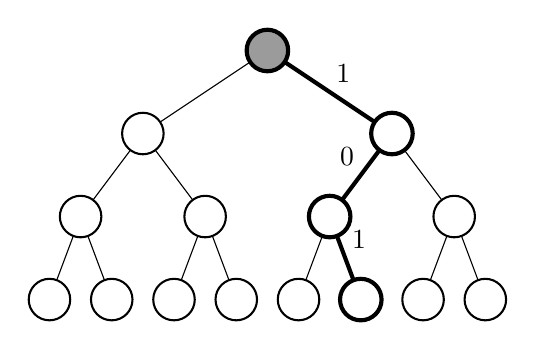
\begin{tikzpicture}[x=0.75pt,y=0.75pt,yscale=-1,xscale=1]
%uncomment if require: \path (0,201); %set diagram left start at 0, and has height of 201

%Straight Lines [id:da918933314477578] 
\draw    (25,90) -- (10,130) ;
%Straight Lines [id:da17752403794816818] 
\draw    (25,90) -- (40,130) ;
%Straight Lines [id:da39739380547431047] 
\draw    (85,90) -- (70,130) ;
%Straight Lines [id:da8176534439302041] 
\draw    (85,90) -- (100,130) ;
%Straight Lines [id:da11119551564082819] 
\draw    (145,90) -- (130,130) ;
%Straight Lines [id:da03948368488437359] 
\draw [line width=1.5]    (145,90) -- (160,130) ;
%Straight Lines [id:da6961629200987864] 
\draw    (205,90) -- (190,130) ;
%Straight Lines [id:da2074079789109078] 
\draw    (205,90) -- (220,130) ;
%Straight Lines [id:da5468814977357803] 
\draw    (55,50) -- (25,90) ;
%Straight Lines [id:da9893002745985011] 
\draw    (55,50) -- (85,90) ;
%Straight Lines [id:da8593115230517709] 
\draw [line width=1.5]    (175,50) -- (145,90) ;
%Straight Lines [id:da23020903575475726] 
\draw    (175,50) -- (205,90) ;
%Straight Lines [id:da03126695179086236] 
\draw    (115,10) -- (55,50) ;
%Straight Lines [id:da3788608056533551] 
\draw [line width=1.5]    (115,10) -- (175,50) ;
%Shape: Circle [id:dp7171076115795707] 
\draw  [fill={rgb, 255:red, 255; green, 255; blue, 255 }  ,fill opacity=1 ][line width=0.75]  (0,130) .. controls (0,124.48) and (4.48,120) .. (10,120) .. controls (15.52,120) and (20,124.48) .. (20,130) .. controls (20,135.52) and (15.52,140) .. (10,140) .. controls (4.48,140) and (0,135.52) .. (0,130) -- cycle ;
%Shape: Circle [id:dp9368220803834215] 
\draw  [fill={rgb, 255:red, 255; green, 255; blue, 255 }  ,fill opacity=1 ][line width=0.75]  (30,130) .. controls (30,124.48) and (34.48,120) .. (40,120) .. controls (45.52,120) and (50,124.48) .. (50,130) .. controls (50,135.52) and (45.52,140) .. (40,140) .. controls (34.48,140) and (30,135.52) .. (30,130) -- cycle ;
%Shape: Circle [id:dp48873250304858695] 
\draw  [fill={rgb, 255:red, 255; green, 255; blue, 255 }  ,fill opacity=1 ][line width=0.75]  (60,130) .. controls (60,124.48) and (64.48,120) .. (70,120) .. controls (75.52,120) and (80,124.48) .. (80,130) .. controls (80,135.52) and (75.52,140) .. (70,140) .. controls (64.48,140) and (60,135.52) .. (60,130) -- cycle ;
%Shape: Circle [id:dp22034783547222947] 
\draw  [fill={rgb, 255:red, 255; green, 255; blue, 255 }  ,fill opacity=1 ][line width=0.75]  (90,130) .. controls (90,124.48) and (94.48,120) .. (100,120) .. controls (105.52,120) and (110,124.48) .. (110,130) .. controls (110,135.52) and (105.52,140) .. (100,140) .. controls (94.48,140) and (90,135.52) .. (90,130) -- cycle ;
%Shape: Circle [id:dp2757783513333645] 
\draw  [fill={rgb, 255:red, 255; green, 255; blue, 255 }  ,fill opacity=1 ][line width=0.75]  (120,130) .. controls (120,124.48) and (124.48,120) .. (130,120) .. controls (135.52,120) and (140,124.48) .. (140,130) .. controls (140,135.52) and (135.52,140) .. (130,140) .. controls (124.48,140) and (120,135.52) .. (120,130) -- cycle ;
%Shape: Circle [id:dp19018674391997514] 
\draw  [fill={rgb, 255:red, 255; green, 255; blue, 255 }  ,fill opacity=1 ][line width=1.5]  (150,130) .. controls (150,124.48) and (154.48,120) .. (160,120) .. controls (165.52,120) and (170,124.48) .. (170,130) .. controls (170,135.52) and (165.52,140) .. (160,140) .. controls (154.48,140) and (150,135.52) .. (150,130) -- cycle ;
%Shape: Circle [id:dp11097581014971603] 
\draw  [fill={rgb, 255:red, 255; green, 255; blue, 255 }  ,fill opacity=1 ][line width=0.75]  (180,130) .. controls (180,124.48) and (184.48,120) .. (190,120) .. controls (195.52,120) and (200,124.48) .. (200,130) .. controls (200,135.52) and (195.52,140) .. (190,140) .. controls (184.48,140) and (180,135.52) .. (180,130) -- cycle ;
%Shape: Circle [id:dp3597073159751265] 
\draw  [fill={rgb, 255:red, 255; green, 255; blue, 255 }  ,fill opacity=1 ][line width=0.75]  (210,130) .. controls (210,124.48) and (214.48,120) .. (220,120) .. controls (225.52,120) and (230,124.48) .. (230,130) .. controls (230,135.52) and (225.52,140) .. (220,140) .. controls (214.48,140) and (210,135.52) .. (210,130) -- cycle ;
%Shape: Circle [id:dp8302463110654139] 
\draw  [fill={rgb, 255:red, 255; green, 255; blue, 255 }  ,fill opacity=1 ][line width=0.75]  (15,90) .. controls (15,84.48) and (19.48,80) .. (25,80) .. controls (30.52,80) and (35,84.48) .. (35,90) .. controls (35,95.52) and (30.52,100) .. (25,100) .. controls (19.48,100) and (15,95.52) .. (15,90) -- cycle ;
%Shape: Circle [id:dp14166594502287744] 
\draw  [fill={rgb, 255:red, 255; green, 255; blue, 255 }  ,fill opacity=1 ][line width=0.75]  (75,90) .. controls (75,84.48) and (79.48,80) .. (85,80) .. controls (90.52,80) and (95,84.48) .. (95,90) .. controls (95,95.52) and (90.52,100) .. (85,100) .. controls (79.48,100) and (75,95.52) .. (75,90) -- cycle ;
%Shape: Circle [id:dp2421410022770858] 
\draw  [fill={rgb, 255:red, 255; green, 255; blue, 255 }  ,fill opacity=1 ][line width=1.5]  (135,90) .. controls (135,84.48) and (139.48,80) .. (145,80) .. controls (150.52,80) and (155,84.48) .. (155,90) .. controls (155,95.52) and (150.52,100) .. (145,100) .. controls (139.48,100) and (135,95.52) .. (135,90) -- cycle ;
%Shape: Circle [id:dp03553548766246628] 
\draw  [fill={rgb, 255:red, 255; green, 255; blue, 255 }  ,fill opacity=1 ][line width=0.75]  (195,90) .. controls (195,84.48) and (199.48,80) .. (205,80) .. controls (210.52,80) and (215,84.48) .. (215,90) .. controls (215,95.52) and (210.52,100) .. (205,100) .. controls (199.48,100) and (195,95.52) .. (195,90) -- cycle ;
%Shape: Circle [id:dp42172995290085846] 
\draw  [fill={rgb, 255:red, 255; green, 255; blue, 255 }  ,fill opacity=1 ][line width=0.75]  (45,50) .. controls (45,44.48) and (49.48,40) .. (55,40) .. controls (60.52,40) and (65,44.48) .. (65,50) .. controls (65,55.52) and (60.52,60) .. (55,60) .. controls (49.48,60) and (45,55.52) .. (45,50) -- cycle ;
%Shape: Circle [id:dp9485260519035812] 
\draw  [fill={rgb, 255:red, 255; green, 255; blue, 255 }  ,fill opacity=1 ][line width=1.5]  (165,50) .. controls (165,44.48) and (169.48,40) .. (175,40) .. controls (180.52,40) and (185,44.48) .. (185,50) .. controls (185,55.52) and (180.52,60) .. (175,60) .. controls (169.48,60) and (165,55.52) .. (165,50) -- cycle ;
%Shape: Circle [id:dp1325104081463544] 
\draw  [fill={rgb, 255:red, 155; green, 155; blue, 155 }  ,fill opacity=1 ][line width=1.5]  (105,10) .. controls (105,4.48) and (109.48,0) .. (115,0) .. controls (120.52,0) and (125,4.48) .. (125,10) .. controls (125,15.52) and (120.52,20) .. (115,20) .. controls (109.48,20) and (105,15.52) .. (105,10) -- cycle ;

% Text Node
\draw (147,26.6) node [anchor=south west] [inner sep=0.75pt]    {$1$};
% Text Node
\draw (158,66.6) node [anchor=south east] [inner sep=0.75pt]    {$0$};
% Text Node
\draw (154.5,106.6) node [anchor=south west] [inner sep=0.75pt]    {$1$};


\end{tikzpicture}
  \caption{$\ell=3$时的评估树。加粗的路径对应于输入$x=101$。根结点被阴影着色,说明它被分配了一个随机标签。所有其他的结点都按照派生规则分配标签。}
  \label{fig:4-15}
\end{figure}

\begin{theorem}\label{theo:4-10}
如果 $G$ 是一个安全的 PRG,那么使用树构造由 $G$ 得到的 PRF $F$ 是一个安全的 PRF。
\begin{quote}
特别地,对于每一个就 $F$ 进行攻击游戏 \ref{game:4-2} 的 PRF 对手 $\mathcal{A}$,如果它最多向挑战者发起 $Q$ 次查询,则必然存在一个就 $G$ 进行攻击游戏 \ref{game:3-1} 的 PRG 对手 $\mathcal{B}$,其中 $\mathcal{B}$ 是一个围绕 $\mathcal{A}$ 的基本包装器,满足:
\end{quote}
\[
{\rm PRF\mathsf{adv}}[\mathcal{A},F]=\ell Q\cdot{\rm PRG\mathsf{adv}}[\mathcal{B},G]
\]
\end{theorem}

\begin{proof}[证明思路]
证明的基本思路是一个混合论证。我们建立一连串的游戏:混合$0$,$\dots$,混合$\ell$。这些游戏中的每一个都是在一个给定的攻击 $F$ 的 PRF 对手和一个挑战者之间进行的,其中挑战者在每个游戏中的行为都略有不同。在混合 $j$ 中,挑战者会构建一颗评估树,其结点按以下方式标记:
\begin{itemize}
	\item 第 $0$ 层到第 $j$ 层的结点会被分配随机标签;
	\item 第 $j+1$ 层到第 $\ell$ 层的结点会被分配派生标签。
\end{itemize}
为了应答混合 $j$ 中的查询 $x\in\{0,1\}^\ell$,挑战者向对手发送由 $x$ 寻址的叶子结点的标签,见图 \ref{fig:4-16}。

\begin{figure}
  \centering
  

\tikzset{every picture/.style={line width=0.75pt}} %set default line width to 0.75pt        

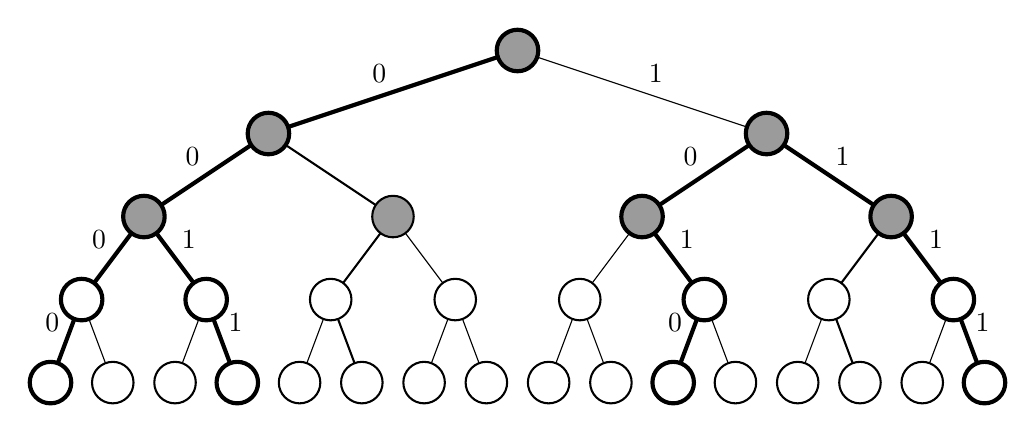
\begin{tikzpicture}[x=0.75pt,y=0.75pt,yscale=-1,xscale=1]
%uncomment if require: \path (0,196); %set diagram left start at 0, and has height of 196

%Straight Lines [id:da18030786969741874] 
\draw [line width=1.5]    (235,10) -- (115,50) ;
%Straight Lines [id:da08184252066372677] 
\draw    (235,10) -- (355,50) ;
%Straight Lines [id:da6695423787123118] 
\draw [line width=1.5]    (25,130) -- (10,170) ;
%Straight Lines [id:da8776558920239244] 
\draw    (25,130) -- (40,170) ;
%Straight Lines [id:da456480770871897] 
\draw    (85,130) -- (70,170) ;
%Straight Lines [id:da24213870313796404] 
\draw [line width=1.5]    (85,130) -- (100,170) ;
%Straight Lines [id:da6422874840426858] 
\draw    (145,130) -- (130,170) ;
%Straight Lines [id:da03506691074715662] 
\draw [line width=0.75]    (145,130) -- (160,170) ;
%Straight Lines [id:da06640681512096891] 
\draw    (205,130) -- (190,170) ;
%Straight Lines [id:da5432180850374912] 
\draw    (205,130) -- (220,170) ;
%Straight Lines [id:da9508663907107122] 
\draw [line width=1.5]    (55,90) -- (25,130) ;
%Straight Lines [id:da9754036077349393] 
\draw [line width=1.5]    (55,90) -- (85,130) ;
%Straight Lines [id:da17473830580335048] 
\draw [line width=0.75]    (175,90) -- (145,130) ;
%Straight Lines [id:da24977957224163605] 
\draw    (175,90) -- (205,130) ;
%Straight Lines [id:da7576985148237267] 
\draw [line width=1.5]    (115,50) -- (55,90) ;
%Straight Lines [id:da42857534612705006] 
\draw [line width=0.75]    (115,50) -- (175,90) ;
%Shape: Circle [id:dp03905566301592911] 
\draw  [fill={rgb, 255:red, 255; green, 255; blue, 255 }  ,fill opacity=1 ][line width=1.5]  (0,170) .. controls (0,164.48) and (4.48,160) .. (10,160) .. controls (15.52,160) and (20,164.48) .. (20,170) .. controls (20,175.52) and (15.52,180) .. (10,180) .. controls (4.48,180) and (0,175.52) .. (0,170) -- cycle ;
%Shape: Circle [id:dp09712081988307864] 
\draw  [fill={rgb, 255:red, 255; green, 255; blue, 255 }  ,fill opacity=1 ][line width=0.75]  (30,170) .. controls (30,164.48) and (34.48,160) .. (40,160) .. controls (45.52,160) and (50,164.48) .. (50,170) .. controls (50,175.52) and (45.52,180) .. (40,180) .. controls (34.48,180) and (30,175.52) .. (30,170) -- cycle ;
%Shape: Circle [id:dp08628380634376609] 
\draw  [fill={rgb, 255:red, 255; green, 255; blue, 255 }  ,fill opacity=1 ][line width=0.75]  (60,170) .. controls (60,164.48) and (64.48,160) .. (70,160) .. controls (75.52,160) and (80,164.48) .. (80,170) .. controls (80,175.52) and (75.52,180) .. (70,180) .. controls (64.48,180) and (60,175.52) .. (60,170) -- cycle ;
%Shape: Circle [id:dp8302838626680549] 
\draw  [fill={rgb, 255:red, 255; green, 255; blue, 255 }  ,fill opacity=1 ][line width=1.5]  (90,170) .. controls (90,164.48) and (94.48,160) .. (100,160) .. controls (105.52,160) and (110,164.48) .. (110,170) .. controls (110,175.52) and (105.52,180) .. (100,180) .. controls (94.48,180) and (90,175.52) .. (90,170) -- cycle ;
%Shape: Circle [id:dp8706292046593302] 
\draw  [fill={rgb, 255:red, 255; green, 255; blue, 255 }  ,fill opacity=1 ][line width=0.75]  (120,170) .. controls (120,164.48) and (124.48,160) .. (130,160) .. controls (135.52,160) and (140,164.48) .. (140,170) .. controls (140,175.52) and (135.52,180) .. (130,180) .. controls (124.48,180) and (120,175.52) .. (120,170) -- cycle ;
%Shape: Circle [id:dp4559690350844394] 
\draw  [fill={rgb, 255:red, 255; green, 255; blue, 255 }  ,fill opacity=1 ][line width=0.75]  (150,170) .. controls (150,164.48) and (154.48,160) .. (160,160) .. controls (165.52,160) and (170,164.48) .. (170,170) .. controls (170,175.52) and (165.52,180) .. (160,180) .. controls (154.48,180) and (150,175.52) .. (150,170) -- cycle ;
%Shape: Circle [id:dp5597760850046549] 
\draw  [fill={rgb, 255:red, 255; green, 255; blue, 255 }  ,fill opacity=1 ][line width=0.75]  (180,170) .. controls (180,164.48) and (184.48,160) .. (190,160) .. controls (195.52,160) and (200,164.48) .. (200,170) .. controls (200,175.52) and (195.52,180) .. (190,180) .. controls (184.48,180) and (180,175.52) .. (180,170) -- cycle ;
%Shape: Circle [id:dp5747757446149799] 
\draw  [fill={rgb, 255:red, 255; green, 255; blue, 255 }  ,fill opacity=1 ][line width=0.75]  (210,170) .. controls (210,164.48) and (214.48,160) .. (220,160) .. controls (225.52,160) and (230,164.48) .. (230,170) .. controls (230,175.52) and (225.52,180) .. (220,180) .. controls (214.48,180) and (210,175.52) .. (210,170) -- cycle ;
%Shape: Circle [id:dp13687363238538053] 
\draw  [fill={rgb, 255:red, 255; green, 255; blue, 255 }  ,fill opacity=1 ][line width=1.5]  (15,130) .. controls (15,124.48) and (19.48,120) .. (25,120) .. controls (30.52,120) and (35,124.48) .. (35,130) .. controls (35,135.52) and (30.52,140) .. (25,140) .. controls (19.48,140) and (15,135.52) .. (15,130) -- cycle ;
%Shape: Circle [id:dp19347578364499673] 
\draw  [fill={rgb, 255:red, 255; green, 255; blue, 255 }  ,fill opacity=1 ][line width=1.5]  (75,130) .. controls (75,124.48) and (79.48,120) .. (85,120) .. controls (90.52,120) and (95,124.48) .. (95,130) .. controls (95,135.52) and (90.52,140) .. (85,140) .. controls (79.48,140) and (75,135.52) .. (75,130) -- cycle ;
%Shape: Circle [id:dp3599355587088173] 
\draw  [fill={rgb, 255:red, 255; green, 255; blue, 255 }  ,fill opacity=1 ][line width=0.75]  (135,130) .. controls (135,124.48) and (139.48,120) .. (145,120) .. controls (150.52,120) and (155,124.48) .. (155,130) .. controls (155,135.52) and (150.52,140) .. (145,140) .. controls (139.48,140) and (135,135.52) .. (135,130) -- cycle ;
%Shape: Circle [id:dp5908856368176647] 
\draw  [fill={rgb, 255:red, 255; green, 255; blue, 255 }  ,fill opacity=1 ][line width=0.75]  (195,130) .. controls (195,124.48) and (199.48,120) .. (205,120) .. controls (210.52,120) and (215,124.48) .. (215,130) .. controls (215,135.52) and (210.52,140) .. (205,140) .. controls (199.48,140) and (195,135.52) .. (195,130) -- cycle ;
%Shape: Circle [id:dp41209359565693915] 
\draw  [fill={rgb, 255:red, 155; green, 155; blue, 155 }  ,fill opacity=1 ][line width=1.5]  (45,90) .. controls (45,84.48) and (49.48,80) .. (55,80) .. controls (60.52,80) and (65,84.48) .. (65,90) .. controls (65,95.52) and (60.52,100) .. (55,100) .. controls (49.48,100) and (45,95.52) .. (45,90) -- cycle ;
%Shape: Circle [id:dp009399054741537904] 
\draw  [fill={rgb, 255:red, 155; green, 155; blue, 155 }  ,fill opacity=1 ][line width=0.75]  (165,90) .. controls (165,84.48) and (169.48,80) .. (175,80) .. controls (180.52,80) and (185,84.48) .. (185,90) .. controls (185,95.52) and (180.52,100) .. (175,100) .. controls (169.48,100) and (165,95.52) .. (165,90) -- cycle ;
%Shape: Circle [id:dp528073778475892] 
\draw  [fill={rgb, 255:red, 155; green, 155; blue, 155 }  ,fill opacity=1 ][line width=1.5]  (105,50) .. controls (105,44.48) and (109.48,40) .. (115,40) .. controls (120.52,40) and (125,44.48) .. (125,50) .. controls (125,55.52) and (120.52,60) .. (115,60) .. controls (109.48,60) and (105,55.52) .. (105,50) -- cycle ;
%Straight Lines [id:da11852362945611472] 
\draw    (265,130) -- (250,170) ;
%Straight Lines [id:da5591497670415919] 
\draw    (265,130) -- (280,170) ;
%Straight Lines [id:da1401309606957788] 
\draw [line width=1.5]    (325,130) -- (310,170) ;
%Straight Lines [id:da6644822016715766] 
\draw    (325,130) -- (340,170) ;
%Straight Lines [id:da615803123899757] 
\draw    (385,130) -- (370,170) ;
%Straight Lines [id:da4594242880739903] 
\draw [line width=0.75]    (385,130) -- (400,170) ;
%Straight Lines [id:da7326524647487114] 
\draw    (445,130) -- (430,170) ;
%Straight Lines [id:da11271665375045803] 
\draw [line width=1.5]    (445,130) -- (460,170) ;
%Straight Lines [id:da6713398753370163] 
\draw    (295,90) -- (265,130) ;
%Straight Lines [id:da9911783089548187] 
\draw [line width=1.5]    (295,90) -- (325,130) ;
%Straight Lines [id:da20755832049249] 
\draw [line width=0.75]    (415,90) -- (385,130) ;
%Straight Lines [id:da6670171480483362] 
\draw [line width=1.5]    (415,90) -- (445,130) ;
%Straight Lines [id:da6886428816533332] 
\draw [line width=1.5]    (355,50) -- (295,90) ;
%Straight Lines [id:da39314609681321877] 
\draw [line width=1.5]    (355,50) -- (415,90) ;
%Shape: Circle [id:dp7753000345940457] 
\draw  [fill={rgb, 255:red, 255; green, 255; blue, 255 }  ,fill opacity=1 ][line width=0.75]  (240,170) .. controls (240,164.48) and (244.48,160) .. (250,160) .. controls (255.52,160) and (260,164.48) .. (260,170) .. controls (260,175.52) and (255.52,180) .. (250,180) .. controls (244.48,180) and (240,175.52) .. (240,170) -- cycle ;
%Shape: Circle [id:dp4802713208709277] 
\draw  [fill={rgb, 255:red, 255; green, 255; blue, 255 }  ,fill opacity=1 ][line width=0.75]  (270,170) .. controls (270,164.48) and (274.48,160) .. (280,160) .. controls (285.52,160) and (290,164.48) .. (290,170) .. controls (290,175.52) and (285.52,180) .. (280,180) .. controls (274.48,180) and (270,175.52) .. (270,170) -- cycle ;
%Shape: Circle [id:dp13339622257445383] 
\draw  [fill={rgb, 255:red, 255; green, 255; blue, 255 }  ,fill opacity=1 ][line width=1.5]  (300,170) .. controls (300,164.48) and (304.48,160) .. (310,160) .. controls (315.52,160) and (320,164.48) .. (320,170) .. controls (320,175.52) and (315.52,180) .. (310,180) .. controls (304.48,180) and (300,175.52) .. (300,170) -- cycle ;
%Shape: Circle [id:dp725595936684422] 
\draw  [fill={rgb, 255:red, 255; green, 255; blue, 255 }  ,fill opacity=1 ][line width=0.75]  (330,170) .. controls (330,164.48) and (334.48,160) .. (340,160) .. controls (345.52,160) and (350,164.48) .. (350,170) .. controls (350,175.52) and (345.52,180) .. (340,180) .. controls (334.48,180) and (330,175.52) .. (330,170) -- cycle ;
%Shape: Circle [id:dp8260566334335642] 
\draw  [fill={rgb, 255:red, 255; green, 255; blue, 255 }  ,fill opacity=1 ][line width=0.75]  (360,170) .. controls (360,164.48) and (364.48,160) .. (370,160) .. controls (375.52,160) and (380,164.48) .. (380,170) .. controls (380,175.52) and (375.52,180) .. (370,180) .. controls (364.48,180) and (360,175.52) .. (360,170) -- cycle ;
%Shape: Circle [id:dp39960075028076947] 
\draw  [fill={rgb, 255:red, 255; green, 255; blue, 255 }  ,fill opacity=1 ][line width=0.75]  (390,170) .. controls (390,164.48) and (394.48,160) .. (400,160) .. controls (405.52,160) and (410,164.48) .. (410,170) .. controls (410,175.52) and (405.52,180) .. (400,180) .. controls (394.48,180) and (390,175.52) .. (390,170) -- cycle ;
%Shape: Circle [id:dp8132641785887298] 
\draw  [fill={rgb, 255:red, 255; green, 255; blue, 255 }  ,fill opacity=1 ][line width=0.75]  (420,170) .. controls (420,164.48) and (424.48,160) .. (430,160) .. controls (435.52,160) and (440,164.48) .. (440,170) .. controls (440,175.52) and (435.52,180) .. (430,180) .. controls (424.48,180) and (420,175.52) .. (420,170) -- cycle ;
%Shape: Circle [id:dp48883984021614624] 
\draw  [fill={rgb, 255:red, 255; green, 255; blue, 255 }  ,fill opacity=1 ][line width=1.5]  (450,170) .. controls (450,164.48) and (454.48,160) .. (460,160) .. controls (465.52,160) and (470,164.48) .. (470,170) .. controls (470,175.52) and (465.52,180) .. (460,180) .. controls (454.48,180) and (450,175.52) .. (450,170) -- cycle ;
%Shape: Circle [id:dp6411714596707287] 
\draw  [fill={rgb, 255:red, 255; green, 255; blue, 255 }  ,fill opacity=1 ][line width=0.75]  (255,130) .. controls (255,124.48) and (259.48,120) .. (265,120) .. controls (270.52,120) and (275,124.48) .. (275,130) .. controls (275,135.52) and (270.52,140) .. (265,140) .. controls (259.48,140) and (255,135.52) .. (255,130) -- cycle ;
%Shape: Circle [id:dp30417580383311815] 
\draw  [fill={rgb, 255:red, 255; green, 255; blue, 255 }  ,fill opacity=1 ][line width=1.5]  (315,130) .. controls (315,124.48) and (319.48,120) .. (325,120) .. controls (330.52,120) and (335,124.48) .. (335,130) .. controls (335,135.52) and (330.52,140) .. (325,140) .. controls (319.48,140) and (315,135.52) .. (315,130) -- cycle ;
%Shape: Circle [id:dp3363829552561317] 
\draw  [fill={rgb, 255:red, 255; green, 255; blue, 255 }  ,fill opacity=1 ][line width=0.75]  (375,130) .. controls (375,124.48) and (379.48,120) .. (385,120) .. controls (390.52,120) and (395,124.48) .. (395,130) .. controls (395,135.52) and (390.52,140) .. (385,140) .. controls (379.48,140) and (375,135.52) .. (375,130) -- cycle ;
%Shape: Circle [id:dp7502474616403281] 
\draw  [fill={rgb, 255:red, 255; green, 255; blue, 255 }  ,fill opacity=1 ][line width=1.5]  (435,130) .. controls (435,124.48) and (439.48,120) .. (445,120) .. controls (450.52,120) and (455,124.48) .. (455,130) .. controls (455,135.52) and (450.52,140) .. (445,140) .. controls (439.48,140) and (435,135.52) .. (435,130) -- cycle ;
%Shape: Circle [id:dp5803858053866973] 
\draw  [fill={rgb, 255:red, 155; green, 155; blue, 155 }  ,fill opacity=1 ][line width=1.5]  (285,90) .. controls (285,84.48) and (289.48,80) .. (295,80) .. controls (300.52,80) and (305,84.48) .. (305,90) .. controls (305,95.52) and (300.52,100) .. (295,100) .. controls (289.48,100) and (285,95.52) .. (285,90) -- cycle ;
%Shape: Circle [id:dp3607270758887733] 
\draw  [fill={rgb, 255:red, 155; green, 155; blue, 155 }  ,fill opacity=1 ][line width=1.5]  (405,90) .. controls (405,84.48) and (409.48,80) .. (415,80) .. controls (420.52,80) and (425,84.48) .. (425,90) .. controls (425,95.52) and (420.52,100) .. (415,100) .. controls (409.48,100) and (405,95.52) .. (405,90) -- cycle ;
%Shape: Circle [id:dp6027653601523095] 
\draw  [fill={rgb, 255:red, 155; green, 155; blue, 155 }  ,fill opacity=1 ][line width=1.5]  (345,50) .. controls (345,44.48) and (349.48,40) .. (355,40) .. controls (360.52,40) and (365,44.48) .. (365,50) .. controls (365,55.52) and (360.52,60) .. (355,60) .. controls (349.48,60) and (345,55.52) .. (345,50) -- cycle ;
%Shape: Circle [id:dp7293505921502836] 
\draw  [fill={rgb, 255:red, 155; green, 155; blue, 155 }  ,fill opacity=1 ][line width=1.5]  (225,10) .. controls (225,4.48) and (229.48,0) .. (235,0) .. controls (240.52,0) and (245,4.48) .. (245,10) .. controls (245,15.52) and (240.52,20) .. (235,20) .. controls (229.48,20) and (225,15.52) .. (225,10) -- cycle ;

% Text Node
\draw (173,26.6) node [anchor=south east] [inner sep=0.75pt]    {$0$};
% Text Node
\draw (297,26.6) node [anchor=south west] [inner sep=0.75pt]    {$1$};
% Text Node
\draw (83,66.6) node [anchor=south east] [inner sep=0.75pt]    {$0$};
% Text Node
\draw (38,106.6) node [anchor=south east] [inner sep=0.75pt]    {$0$};
% Text Node
\draw (15.5,146.6) node [anchor=south east] [inner sep=0.75pt]    {$0$};
% Text Node
\draw (323,66.6) node [anchor=south east] [inner sep=0.75pt]    {$0$};
% Text Node
\draw (315.5,146.6) node [anchor=south east] [inner sep=0.75pt]    {$0$};
% Text Node
\draw (72,106.6) node [anchor=south west] [inner sep=0.75pt]    {$1$};
% Text Node
\draw (94.5,146.6) node [anchor=south west] [inner sep=0.75pt]    {$1$};
% Text Node
\draw (312,106.6) node [anchor=south west] [inner sep=0.75pt]    {$1$};
% Text Node
\draw (387,66.6) node [anchor=south west] [inner sep=0.75pt]    {$1$};
% Text Node
\draw (432,106.6) node [anchor=south west] [inner sep=0.75pt]    {$1$};
% Text Node
\draw (454.5,146.6) node [anchor=south west] [inner sep=0.75pt]    {$1$};


\end{tikzpicture}
  \caption{混合$2$中$\ell=4$时的评估树。被阴影着色的结点被分配了随机标签,未被着色的结点被分配了派生标签。加粗的路径对应于输入 $0000$,$0011$,$1010$ 和 $1111$。}
  \label{fig:4-16}
\end{figure}

显然,混合 $0$ 等同于攻击游戏 \ref{game:4-2} 的实验 $0$,而混合 $\ell$ 等同于实验 $1$。直观地说,在假设 $G$ 是一个安全的 PRG 的情况下,对于 $j=0,\dots,\ell-1$,对手应该无法分辨混合 $j$ 和混合 $j+1$。在严格表述这一想法的时候,我们必须要注意,评估树可能是非常巨大的,为了建立一个有效的攻击 $G$ 的 PRG 对手,我们无法负担写下整棵树的开销(甚至是写下树中的一层的开销)。相对地,我们需要利用这样一个事实,即如果 PRF 对手最多向其挑战者发起 $Q$ 次查询(这是一个多项式边界的值),那么在评估树的任何一层 $j$,这 $Q$ 次查询所跟踪的路径最多会涉及 $Q$ 个 $j$ 层中的结点(在图 \ref{fig:4-16} 中,对于给定的输入,应当是第$2$层的第一、第三和第四个结点)。我们构建的 PRG 对手会根据需要使用``忠实的侏儒"思路的一个变体来有效地维护第 $j$ 层的相关随机标签。
\end{proof}

\begin{proof}
令 $\mathcal{A}$ 是一个有效对手,它就 $F$ 进行攻击游戏 \ref{game:4-2} 中的攻击。我们假设 $\mathcal{A}$ 最多向其挑战者发起 $Q$ 次查询,其中 $Q$ 是一个多项式边界的值。

如上所述,我们定义 $\ell+1$ 个混合游戏:混合$0$,$\dots$,混合$\ell$,其中每个游戏都在 $\mathcal{A}$ 和一个挑战者之间进行。在混合 $j$ 中,挑战者的工作方式如下:

\vspace{5pt}

\hspace*{5pt} 选取 $f\overset{\rm R}\leftarrow{\rm Funs}[\{0,1\}^j,\mathcal{S}]$\\
\hspace*{26pt} 当从 $\mathcal{A}$ 处收到查询 $x=(a_1,\dots,a_\ell)\in\{0,1\}^\ell$ 时:\\
\hspace*{50pt} 令 $u\leftarrow(a_1,\dots,a_j)$,$v\leftarrow(a_{j+1},\dots,a_\ell)$\\
\hspace*{50pt} 令 $y\leftarrow G^*(f(u),v)$\\
\hspace*{50pt} 将 $y$ 发送给 $\mathcal{A}$。

\vspace{5pt}

\noindent
直观地说,对于 $u\in\{0,1\}^j$,$f(u)$ 代表 $u$ 所寻址的第 $j$ 层结点的随机标签。因此,第 $j$ 层的每个结点都会被分配一个随机标签,而第 $j+1$ 层到第 $l$ 层的结点都会被分配派生标签。请注意,在我们对混合游戏的描述中,我们没有明确地给第 $0$ 层到第 $j-1$ 层的结点分配标签,因为这些标签不影响任何输出。

对于 $j=0,\dots,\ell$,由于混合 $0$ 相当于攻击游戏 \ref{game:4-2} 的实验 $0$,而混合 $\ell$ 相当于实验 $1$,我们有:
\begin{equation}\label{eq:4-30}
{\rm PRF\mathsf{adv}}[\mathcal{A},F]=|p_\ell-p_0|
\end{equation}

用 $G'$ 表示 $G$ 的 $Q$ 次并行组合,如我们在 \ref{subsec:3-4-1} 小节中介绍过的那样。$G'$ 以 $(s_1,\dots,s_Q)\in\mathcal{S}^Q$ 为输入,输出 $(G(s_1),\dots,G(s_Q))\in(\mathcal{S}^2)^Q$。根据定理 \ref{theo:3-2},如果 $G$ 是一个安全的 PRG,那么 $G'$ 也是一个安全的 PRG。

现在,我们建立一个有效 PRG 对手 $\mathcal{B}'$ 来攻击 $G'$,使得:
\begin{equation}\label{eq:4-31}
{\rm PRG\mathsf{adv}}[\mathcal{B}',G']=\frac{1}{\ell}\cdot|p_\ell-p_0|
\end{equation}
我们首先概述 $\mathcal{B}'$ 的工作原理。在针对 $G'$ 进行攻击游戏 \ref{game:3-1} 中的攻击时,挑战者向 $\mathcal{B}'$ 提出一个向量:
\begin{equation}\label{eq:4-32}
\vec{r}=((r_{10},r_{11}),\dots,(r_{Q0},r_{Q1}))\in(\mathcal{S}^2)^Q
\end{equation}
在攻击游戏的实验 $0$ 中,对于随机的 $\vec{s}\in\mathcal{S}^Q$,有 $\vec{r}=G(\vec{s})$。而在实验 $1$ 中,$\vec{r}$ 是从 $(\mathcal{S}^2)^Q$ 中随机选出的。为了区分这两个实验,$\mathcal{B}'$ 随机选择一个 $\omega\in\{1,\dots,\ell\}$,并扮演 $\mathcal{A}$ 的挑战者的角色,并使用 $\vec r$ 的元素按顺序给评估树的第 $\omega$ 层的结点打上标签。为此,$\mathcal{B}'$ 需要维护一张查找表,这使得它可以将每某个查询 $x\in\{0,1\}^\ell$ 的每个前缀 $u\in\{0,1\}^{\omega-1}$ 与一个索引 $p$ 关联起来,这样,由 $u$ 寻址的结点的子结点就被种子对 $(r_{p0},r_{p1})$ 标记。最后,当 $\mathcal{A}$ 终止并输出一个比特时,$\mathcal{B}'$ 就输出相同的比特。从 $\mathcal{B}'$ 的构造细节可以看出,对于任何固定的 $j=1,\dots,\ell$,以 $\omega=j$ 为条件,$\mathcal{B}'$ 输出 $1$ 的概率为:
\begin{itemize}
	\item $p_{j-1}$,如果 $\mathcal{B}'$ 处于其攻击游戏的实验 $0$ 中,或
	\item $p_j$,如果 $\mathcal{B}'$ 处于其攻击游戏的实验 $1$ 中。
\end{itemize}
然后通过简单的放缩计算,我们就能得到式 \ref{eq:4-31}。

下面我们来说说细节。我们将查找表实现为一个关联数组 $Map:\{0,1\}^*\to\mathbb{Z}_{>0}$。下面是 $\mathcal{B}'$ 的工作原理:

\vspace{5pt}

\hspace*{5pt} 当从挑战者处收到如式 \ref{eq:4-32} 的向量 $\vec r$ 时,$\mathcal{B}'$ 扮演 $\mathcal{A}$ 的挑战者的角色,如下所示:\\
\hspace*{50pt} 选取 $\omega\overset{\rm R}\leftarrow\{1,\dots,\ell\}$\\
\hspace*{50pt} 初始化一个空关联数组 $Map:\{0,1\}^*\to\mathbb{Z}_{>0}$\\
\hspace*{50pt} 令 $ctr\leftarrow 0$\\
\hspace*{50pt} 当从 $\mathcal{A}$ 处收到一个查询 $x=(a_1,\dots,a_\ell)\in\{0,1\}^\ell$ 时:\\
\hspace*{75pt} 令 $u\leftarrow(a_1,\dots,a_{\omega-1})$,$d\leftarrow a_\omega$,$v\leftarrow(a_{\omega+1},\dots,a_\ell)$\\
\hspace*{75pt} 如果 $u\notin{\rm Domain}(Map)$:\\
\hspace*{100pt} 令 $ctr\leftarrow ctr+1$,$Map[u]\leftarrow ctr$\\
\hspace*{75pt} 令 $p\leftarrow Map[u]$,$y\leftarrow G^*(r_{pd},v)$\\
\hspace*{75pt} 将 $y$ 发送给 $\mathcal{A}$。

\vspace{3pt}

\hspace*{5pt} 最后,$\mathcal{B}'$ 输出 $\mathcal{A}$ 所输出的任何东西。

\vspace{5pt}

对于$b=0,1$,令 $W_b$ 为 $\mathcal{B}'$ 就 $G'$ 在攻击游戏 \ref{game:3-1} 的实验 $b$ 中输出 $1$ 的事件。我们声称,对于任何固定的 $j=1,\dots,\ell$,都有:
\[
\Pr[W_0|\omega=j]=p_{j-1},~~~~
\Pr[W_1|\omega=j]=p_j
\]
事实上,以 $\omega=j$ 为条件,对于固定的 $j$,考虑 $\mathcal{B}'$ 如何给评估树中的结点加标签。一方面,当 $\mathcal{B}'$ 处于其攻击游戏的实验 $1$ 时,它可以有效地给第 $j$ 层的结点分配随机标签,而查找表能够确保这些标签不会重复。另一方面,当 $\mathcal{B}'$ 处于其攻击游戏的实验 $0$ 时,它可以有效地给第 $j$ 层的结点分配伪随机标签,这等于给这些结点在第 $j-1$ 层的父结点分配随机标签,并在第 $j$ 层分配派生标签;同样,查找表能够确保标签不会重复。

基于上述声称,我们可以通过一个简单的放缩计算得到式 \ref{eq:4-31}:
\[
\begin{aligned}
{\rm PRG\mathsf{adv}}[\mathcal{B}',G']
&=|\Pr[W_1]-\Pr[W_0]|\\
&=\frac{1}{\ell}\cdot\Big\lvert\sum_{j=1}^\ell\Pr[W_1\,|\,\omega=j]-\sum_{j=1}^\ell\Pr[W_0\,|\,\omega=j]\Big\rvert\\
&=\frac{1}{\ell}\cdot\Big\lvert\sum_{j=1}^\ell p_j-\sum_{j=1}^\ell p_{j-1}\Big\rvert\\
&=\frac{1}{\ell}\cdot|p_\ell-p_0|
\end{aligned}
\]

最后,根据定理 \ref{theo:3-2},必然存在一个有效 PRG 对手 $\mathcal{B}$,使得:
\begin{equation}\label{eq:4-33}
{\rm PRG\mathsf{adv}}[\mathcal{B}',G']=Q\cdot{\rm PRG\mathsf{adv}}[\mathcal{B},G]
\end{equation}
现在,结合式 \ref{eq:4-30},\ref{eq:4-31} 和 \ref{eq:4-33},可以得到该定理。
\end{proof}

\subsection{变长树构造}

很自然地,我们下面考虑树构造如何在可变长度的输入上工作。和之前一样,令 $G$ 是一个定义在 $(\mathcal{S},\mathcal{S}^2)$ 上的 PRG,$G^*$ 的定义与之前也一样。对于任何多项式边界值 $\ell$,我们定义 PRF $\tilde F$,其密钥空间为 $\mathcal{S}$,输入空间为 $\{0,1\}^{\leq l}$,输出空间为 $\mathcal{S}$,对于 $s\in\mathcal{S}$ 和 $x\in\{0,1\}^{\leq\ell}$,我们定义:
\[
\tilde F(s,x)=G^*(s,x)
\]

不幸的是,$\tilde F$ 不是一个安全的 PRF,原因是存在着一种平凡的\textbf{扩展攻击 (extension attack)}。假设 $u,v\in\{0,1\}^{\leq\ell}$,其中 $u$ 是 $v$ 的真前缀,即存在非空序列 $w$ 使得 $v=u\,\Vert\,w$。那么,给定 $u$,$v$ 以及 $y:=\tilde F(s,u)$,我们很容易基于 $G^*(y,w)$ 计算 $F(s,v)$。当然,对于一个真随机函数来说,给定 $u$ 处的值,我们无法预测它在 $v$ 处的值。因此,我们很容易将 $\tilde F(s,\cdot)$ 与一个真随机函数区分开来。

即便 $\tilde F$ 不是一个安全的 PRF,我们仍然可以得出一些关于它的有趣结论。我们下面表明,针对特定的受限对手所组成的集合,$\tilde F$ 是一个 PRF,这种对手被称为\textbf{无前缀对手 (prefix-free adversaries)}。

\begin{definition}\label{def:4-5}
令 $F$ 是一个定义在 $(\mathcal{K},\mathcal{X}^{\leq\ell}, \mathcal{Y})$ 上的 PRF。对于一个就 $F$ 进行攻击游戏 \ref{game:4-2} 中的攻击的 PRF 对手 $\mathcal{A}$,如果它所发出的所有查询都是 $\mathcal{X}$ 上长度不超过 $\ell$ 的非空序列,且其中任何一个查询都不是其他查询的真前缀\footnote[3]{对于序列 $x=(a_1\dots a_s)$ 和 $y=(b_1\dots b_t)$,如果 $s\leq t$,且对于 $i=1,\dots,s$ 都有 $a_i=b_i$,我们就称 $x$ 是 $y$ 的一个\textbf{前缀};在此基础上,如果 $s<t$,我们就称 $x$ 是 $y$ 的一个\textbf{真前缀(proper prefix)}。},我们就称这样的对手 $\mathcal{A}$ 是一个\textbf{无前缀对手 (prefix-free adversary)}。我们将 $\mathcal{A}$ 赢得游戏的优势记为 ${\rm PRF^{pf}\mathsf{adv}}[\mathcal{A},F]$。此外,如果对于所有有效的无前缀对手 $\mathcal{A}$,${\rm PRF^{pf}\mathsf{adv}}[\mathcal{A},F]$ 的值都可忽略不计,我们就称 $F$ 是一个\textbf{无前缀安全的 PRF (prefix-free secure PRF)}。
\end{definition}

比如,如果一个无前缀对手对序列 $(a_1,a_2,a_3)$ 发起查询,那么它就不能再对 $(a_1)$ 和 $(a_1,a_2)$ 发起查询。

\begin{theorem}\label{theo:4-11}
如果 $G$ 是一个安全 PRG,那么由 $G$ 派生的变长树构造 $\tilde F$ 是一个无前缀安全的 PRF。
\begin{quote}
特别地,对于每个就 $\tilde F$ 进行攻击游戏 \ref{game:4-2} 的无前缀对手 $\mathcal{A}$,如果它最多能向其挑战者发起 $Q$ 次查询,那么必然存在一个就 $G$ 进行攻击游戏 \ref{game:3-1} 的 PRG 对手 $\mathcal{B}$,其中 $\mathcal{B}$ 是一个围绕 $\mathcal{A}$ 的基本包装器,满足:
\end{quote}
\[
{\rm PRF^{pf}\mathsf{adv}}[\mathcal{A},\tilde{F}]=\ell Q\cdot{\rm PRG\mathsf{adv}}[\mathcal{B},G]
\]
\end{theorem}

\begin{proof}
该证明的基本思路与定理 \ref{theo:4-10} 完全相同。我们在此仅简述主要观点,并强调与那个证明的不同之处。

令 $\mathcal{A}$ 是一个有效的无前缀对手,它就 $\tilde F$ 进行攻击游戏 \ref{game:4-2}。假设 $\mathcal{A}$ 最多向其挑战者发起 $Q$ 次查询。此外,为了方便起见,我们假设 $\mathcal{A}$ 发起的任意两次查询都不相同,也不会出现其中一个是另一个的前缀的情况。攻击游戏 \ref{game:4-2} 中的挑战者不需要强制服从这一假设,我们只是假设 $\mathcal{A}$ 在按规则行事。

和之前一样,我们用一棵评估树来考察 $\tilde F(s,\cdot)$ 的计算:其根结点的标签为 $s$,所有其他结点的标签都是派生标签。现在唯一的区别是,$\tilde F(s,\cdot)$ 的输入也可以寻址到评估树的\emph{内部}结点。然而,无前缀的约束意味着,没有任何一个输入可以寻址到一个由之前输入所寻址的结点的祖先结点。

我们再次定义 $\ell$ 个混合游戏:混合$0$,$\dots$,混合$\ell$。在这些游戏中,挑战者使用的评估树的标记方式与定理 \ref{theo:4-10} 的证明中完全相同:在混合 $j$ 中,第 $0$ 层到第 $j$ 层的结点被分配随机标签,而其他层的结点被分配派生标签。挑战者对查询 $x$ 的应答是返回评估树中 $x$ 所寻址的结点的标签,注意该结点现在不一定是叶子结点。更正式地说,混合 $j$ 中的挑战者的工作方式如下:

\vspace{5pt}

\hspace*{5pt} 选取 $f\overset{\rm R}\leftarrow{\rm Funs}[\{0,1\}^{\leq j},\mathcal{S}]$\\
\hspace*{26pt} 当从 $\mathcal{A}$ 处收到查询 $x=(a_1,\dots,a_n)\in\{0,1\}^\ell$ 时:\\
\hspace*{50pt} 如果 $n<j$:\\
\hspace*{75pt} 则令 $y\leftarrow f(x)$\\
\hspace*{75pt} 否则令 $u\leftarrow(a_1,\dots,a_j)$,$v\leftarrow(a_{j+1},\dots,a_n)$,$y\leftarrow G^*(f(u),v)$\\
\hspace*{50pt} 将 $y$ 发送给 $\mathcal{A}$。

\vspace{5pt}

\noindent
对于$j=0,\dots,l$,定义 $p_j$ 为 $\mathcal{A}$ 在混合 $j$ 中输出 $1$ 的概率。读者很容易验证,我们有:
\[
{\rm PRF^{pf}\mathsf{adv}}[\mathcal{A},\tilde{F}]=|p_\ell-p_0|
\]

接下来,我们定义一个攻击 $G$ 的 $Q$ 次并行组合 $G'$ 的有效 PRG 对手 $\mathcal{B}'$,使得:
\[
{\rm PRG}\mathsf{adv}[\mathcal{B}',G']=\frac{1}{\ell}\cdot|p_\ell-p_0|
\]
对手 $\mathcal{B}'$ 的工作方式如下:

\vspace{5pt}

\hspace*{5pt} 当从挑战者处收到如式 \ref{eq:4-32} 的向量 $\vec r$ 时,$\mathcal{B}'$ 扮演 $\mathcal{A}$ 的挑战者的角色,如下所示:\\
\hspace*{50pt} 选取 $\omega\overset{\rm R}\leftarrow\{1,\dots,\ell\}$\\
\hspace*{50pt} 初始化一个空关联数组 $Map:\{0,1\}^*\to\mathbb{Z}_{>0}$\\
\hspace*{50pt} 令 $ctr\leftarrow 0$\\
\hspace*{50pt} 当从 $\mathcal{A}$ 处收到一个查询 $x=(a_1,\dots,a_n)\in\{0,1\}^\ell$ 时:\\
\hspace*{75pt} 如果 $n<\omega$:\\
\hspace*{11pt} ($*$)
\hspace*{69pt} 选取 $y\overset{\rm R}\leftarrow\mathcal{S}$\\
\hspace*{75pt} 否则:\\
\hspace*{100pt} 令 $u\leftarrow(a_1,\dots,a_{\omega-1})$,$d\leftarrow a_\omega$,$v\leftarrow(a_{\omega+1},\dots,a_n)$\\
\hspace*{100pt} 如果 $u\notin{\rm Domain}(Map)$:\\
\hspace*{125pt} 令 $ctr\leftarrow ctr+1$,$Map[u]\leftarrow ctr$\\
\hspace*{100pt} 令 $p\leftarrow Map[u]$,$y\leftarrow G^*(r_{pd},v)$\\
\hspace*{75pt} 将 $y$ 发送给 $\mathcal{A}$。

\vspace{3pt}

\hspace*{5pt} 最后,$\mathcal{B}'$ 输出 $\mathcal{A}$ 所输出的任何东西。

\vspace{5pt}

对于 $b=0,1$,记 $W_b$ 为 $\mathcal{B}'$ 就 $G'$ 在攻击游戏 \ref{game:4-2} 的实验 $b$ 中输出 $1$ 的事件。不难看出,对于任意固定的 $j=1,\dots,\ell$,我们有:
\[
\Pr[W_0|\omega=j]=p_{j-1},~~~~
\Pr[W_1|\omega=j]=p_j
\]
事实上,以 $\omega=j$ 为条件,对于固定的 $j$,考察 $\mathcal{B}'$ 如何给评估树中的结点加上标签。在标有($*$)的那一行,$\mathcal{B}'$ 给评估树中第 $0$ 层到第 $j-1$ 层的所有结点都分配了随机标签。由于我们假设 $\mathcal{A}$ 不会发起两次同样的查询,因此同一个结点不会在不同时间收到两个不同的标签。现在,一方面,当 $\mathcal{B}'$ 处于其攻击游戏的实验 $1$ 时,它可以有效地给第 $j$ 层的结点分配随机标签,而查找表能够确保不会出现重复。另一方面,当 $\mathcal{B}'$ 处于其攻击游戏的实验 $0$ 时,它可以有效地给第 $j$ 层的结点分配伪随机标签,这等同于给这些结点在第 $j-1$ 层的父结点分配随机标签;而无前缀的假设能够保证,在标有($*$)的那一行,这些父结点中的任何一个都不会被赋予已经分配出去的标签。

证明的剩余部分与定理 \ref{theo:4-10} 相同,不再赘述。
\end{proof}